\documentclass[11pt,spanish]{article}

\usepackage[spanish]{babel}
\usepackage[utf8]{inputenc}
\usepackage{fancyhdr} % Required for custom headers
\usepackage{lastpage} % Required to determine the last page for the footer
\usepackage{extramarks} % Required for headers and footers
\usepackage{graphicx} % Required to insert images
\usepackage{lipsum} % Used for inserting dummy 'Lorem ipsum' text into the template


% Margins
\topmargin=-0.35in
\evensidemargin=0in
\oddsidemargin=0in
\textwidth=6.5in
\textheight=9.0in
\headsep=0.25in 

\linespread{1.1} % Line spacing

% Set up the header and footer
\pagestyle{fancy}% Top left header
\rhead{} % Top right header
\lfoot{\lastxmark} % Bottom left footer
\cfoot{} % Bottom center footer
\rfoot{P\'{a}gina\ \thepage\ de\ \pageref{LastPage}} % Bottom right footer
\renewcommand\headrulewidth{0.4pt} % Size of the header rule
\renewcommand\footrulewidth{0.4pt} % Size of the footer rule

\setlength\parindent{0pt} % Removes all indentation from paragraphs

%----------------------------------------------------------------------------------------
%	DOCUMENT STRUCTURE COMMANDS
%	Skip this unless you know what you're doing
%----------------------------------------------------------------------------------------



\setcounter{secnumdepth}{0} % Removes default section numbers
\newcounter{homeworkProblemCounter} % Creates a counter to keep track of the number of problems

\newcommand{\homeworkProblemName}{}
\newenvironment{homeworkProblem}[1][Parte \arabic{homeworkProblemCounter}]{ % Makes a new environment called homeworkProblem which takes 1 argument (custom name) but the default is "Problem #"
\stepcounter{homeworkProblemCounter} % Increase counter for number of problems
\renewcommand{\homeworkProblemName}{#1} % Assign \homeworkProblemName the name of the problem
\section{\homeworkProblemName} % Make a section in the document with the custom problem count

}

\newcommand{\problemAnswer}[1]{ % Defines the problem answer command with the content as the only argument
\noindent\framebox[\columnwidth][c]{\begin{minipage}{0.98\columnwidth}#1\end{minipage}} % Makes the box around the problem answer and puts the content inside
}

\newcommand{\homeworkSectionName}{}
\newenvironment{homeworkSection}[1][Parte \arabic{homeworkProblemCounter}]{ % New environment for sections within homework problems, takes 1 argument - the name of the section
\renewcommand{\homeworkSectionName}{#1} % Assign \homeworkSectionName to the name of the section from the environment argument
\subsection{\homeworkSectionName} % Make a subsection with the custom name of the subsection
}{
}
   
%----------------------------------------------------------------------------------------
%	NAME AND CLASS SECTION
%----------------------------------------------------------------------------------------

\newcommand{\hmwkTitle}{Empresa XXX S.A.} % Assignment title
\newcommand{\hmwkDueDate}{Mi\'{e}rcoles,\ Mayo\ 25,\ 2016} % Due date
\newcommand{\hmwkClass}{GC} % Course/class
\newcommand{\hmwkClassInstructor}{Maria Jose Gils} % Teacher/lecturer
\newcommand{\hmwkAuthorName}{Gorka Barturen y Carlos Perales} % Your name

%----------------------------------------------------------------------------------------
%	TITLE PAGE
%----------------------------------------------------------------------------------------

\title{
\vspace{2in}
\textmd{\textbf{\hmwkClass:\ \hmwkTitle}}\\
\normalsize\vspace{0.1in}\small{\hmwkDueDate}\\
\vspace{3in}
}

\author{\textbf{\hmwkAuthorName}}
\date{} % Insert date here if you want it to appear below your name

%----------------------------------------------------------------------------------------

\begin{document}

\maketitle

%----------------------------------------------------------------------------------------
%	TABLE OF CONTENTS
%----------------------------------------------------------------------------------------

%\setcounter{tocdepth}{1} % Uncomment this line if you don't want subsections listed in the ToC

\newpage
\tableofcontents
\newpage

%----------------------------------------------------------------------------------------
%	PROBLEM 1
%----------------------------------------------------------------------------------------

% To have just one problem per page, simply put a \clearpage after each problem

\begin{homeworkProblem}[1.1. Visi\'{o}n, Misi\'{o}n y estrategia]
Visi\'{o}n:
\begin{itemize}

\item Ser la empresa l\'{i}der en Espa\~{n}a en la venta de electrodom\'{e}sticos.
\item Ser una empresa que trabaje tanto por la sostenibilidad de s\'{i} misma como por la de sus productos.
\item Ampliar la infraestructura de la empresa a nivel internacional.
\item Mejora del ciclo de vida de los productos.

\end{itemize}

Misi\'{o}n: Ser la empresa que produce los electrodom\'{e}sticos sostenibles con mejor relaci\'{o}n calidad-precio.

\end{homeworkProblem}
\clearpage

%----------------------------------------------------------------------------------------
%	PROBLEM 2
%----------------------------------------------------------------------------------------
\begin{homeworkProblem}[1.2. Identificaci\'{o}n de los conocimientos pertinentes ]

\begin{homeworkSection}[a. Auditor\'{i}a del conocimiento inicial]  % Custom section title
Auditor\'{i}a de sistemas:
\begin{itemize}

\item SAP  (Sistema ERP): conocimiento del funcionamiento tanto de la empresa como de los clientes y proveedores.
\item Oracle (SGBD): conocimiento guardado en las bases de datos de los diferentes departamentos (empleados, productos…)
\item Procesadores de textos 
\item Intranet/Extranet:  conocimiento general tanto de la empresa como del empleado que la consulta


\end{itemize}

Auditor\'{i}a de personas:

\begin{itemize}

\item Accionistas de la asamblea general
\item Miembros de la asamblea permanente
\item Director general
\item Representantes de cada departamento
\item Empleados de cada departamento

\end{itemize}

Auditor\'{i}a de procesos:

\begin{itemize}

\item Fabricación de productos
\item Creación de un nuevo producto: conocimiento de las necesidades del mercado para la adecuación de un nuevo producto
\item Venta de productos: conocimiento tanto de los clientes como de nuestros productos
\item Compra de materiales: conocimiento de los materiales que necesitamos para garantizar la calidad de nuestros productos
\item Contratación de empleados: conocimiento de los empleados para la adecuación a los puestos 


\end{itemize}

\end{homeworkSection}
\clearpage

%----------------------------------------------------------------------------------------
%	PROBLEM 3
%----------------------------------------------------------------------------------------

\begin{homeworkSection}[b. An\'{a}lisis DAFO] % 
Debilidades:
\begin{itemize}

\item A pesar de ser reconocidos en España, no tenemos demasiado mercado fuera del pa\'{i}s
\item Alto coste de fabricaci\'{o}n para mantener nuestra calidad

\end{itemize}

Amenazas:

\begin{itemize}

\item Que otras empresas compitan contra nosotros centr\'{a}ndose en nuestra ventaja competitiva y bajen los costes del producto
\item Que no consigamos expandirnos fuera de Espa\~{n}a por alg\'{u}n problema de legislaci\'{o}n.

\end{itemize}

Fortalezas:

\begin{itemize}

\item Somos una marca referente en Espa\~{n}a
\item Diferentes gamas de productos para satisfacer a diferentes consumidores

\end{itemize}

Oportunidades:

\begin{itemize}

\item Nuevos mercados con necesidades b\'{a}sicas que cubrimos gracias a nuestra amplia gama de productos

\end{itemize}



\textbf{Iniciativas de Gesti\'{o}n de Conocimiento}
\begin{itemize}

\item Hacer las p\'{a}ginas amarillas con el conocimiento de cada empleado, estableciendo as\'{i} un documento que recoge todos los perfiles de conocimiento de la empresa para futuras formaciones de grupos y b\'{u}squeda de requisitos en la empresa.



\begin{enumerate}

\item Creación de la aplicación para páginas amarillas
\item Recoger el conocimiento de los empleados


\end{enumerate}

\item Potenciar el mercado internacional aprovechando los mercados emergentes y nuestra amplia gama de productos. 

\begin{enumerate}

\item Analizar los perfiles de los empleados para escoger a los componentes de un equipo que se centrará en el análisis de los diferentes mercados y en valorar los riesgos y los beneficios a la hora de expandirse a un nuevo mercado.

\item Establecer un equipo de adaptación de mercado, que establezca un plan para poder adaptar nuestra empresa a las necesidades del nuevo mercado a la hora de expandirnos. 
Este equipo se encargará también de la búsqueda de debilidades en los mercados, aprovechando las oportunidades que dejan otras empresas para poder impulsarnos de forma más efectiva en estos nuevos mercados.

\end{enumerate}

\item Conseguir que nuestra ventaja competitiva resida en la calidad, de esta forma no habrá ningún problema en competencia de costes


\item Potenciar el mercado internacional aprovechando los mercados emergentes y nuestra amplia gama de productos. 

\begin{enumerate}

\item Analizar los perfiles de los empleados para elegir a los expertos en procesos de calidad o para establecer grupos de formación en procesos de calidad.

\item Establecer un equipo de empleados que analice y monitorice nuestro proceso de calidad para poder reforzarlos, mejorando así la calidad de nuestros productos.


\end{enumerate}


\item Llevar al día los permisos y legislaciones de los nuevos mercados internacionales a los que nos queramos expandir.




\end{itemize}

\end{homeworkSection}
\clearpage

%------------------------------------------------------------------------

\begin{homeworkSection}[c. P\'{a}ginas amarillas] % Custom section title

\begin{itemize}


\item ¿D\'{o}nde guardaremos esta informaci\'{o}n?\\
La informaci\'{o}n de cada empleado estar\'{a} guardada en una base de datos relacional en la que se dividir\'{a}n todos estos datos en tablas, manteniendo as\'{i} un registro ordenado sobre cada una de las caracter\'{i}sticas de los empleados.
\item ¿De d\'{o}nde recogemos la informaci\'{o}n?\\
La informaci\'{o}n de los perfiles de este documento se recoger\'{a} y se actualizar\'{a} desde la base de datos del departamento de recursos humanos, por lo que los empleados no ser\'{a}n los encargados de introducir esta informaci\'{o}n.
\item ¿C\'{o}mo accederemos a ella?\\
Se podr\'{a} acceder a todas las fichas de empleados y a su informaci\'{o}n mediante un buscador, en el cual se filtrar\'{a} la b\'{u}squeda mediante diferentes m\'{e}todos (nombre, proyecto, cursos, tags de conocimiento…) y se visualizar\'{a} una lista de resultados en forma de fichas de empleados que pasen los filtros.
Tambi\'{e}n se puede acceder a informaci\'{o}n sobre cursos, departamentos, proyectos… desde los hiperv\'{i}nculos de la propia ficha del empleado desde la cual se redirigir\'{a} al usuario a la informaci\'{o}n buscada.

\begin{center}
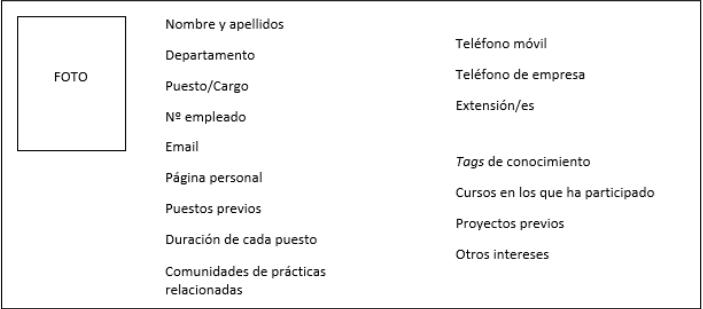
\includegraphics[width=0.85\columnwidth]{PA} % Example image
\end{center}
\end{itemize}
\end{homeworkSection}
\clearpage

%--------------------------------------------

\begin{homeworkSection}[d. Lista de procesos] 

\begin{itemize}
\item (E)An\'{a}lisis de la trayectoria a nivel nacional de la empresa (buenas pr\'{a}cticas)
\item (E)Satisfacci\'{o}n de los empleados
\item (E)An\'{a}lisis y reducci\'{o}n del impacto medioambiental del proceso de producci\'{o}n 
\\

\item (O)Captura del conocimiento de los empleados
\item (O)Proceso de fabricación de electrodomésticos
\item (O)Formaci\'{o}n / Adecuaci\'{o}n de los empleados a los puestos
\\

\item (S)Gesti\'{o}n adecuada de nuestros empleados
\item (S)Atención al cliente
\item (S)Atenci\'{o}n a las sugerencias y reclamaciones (clientes y empleados)

\end{itemize}
\end{homeworkSection}
\clearpage

%----------------------------------------------------------------------------------------

%----------------------------------------------------------------------------------------

\begin{homeworkSection}[e. Definici\'{o}n de procesos ]
\begin{center}
Captura del conocimiento de nuestros empleados

\begin{itemize}

\item Objetivos:  Mantener la base de datos de nuestros empleados actualizada
\item Inicio: Fin de trimestre
\item Fin: Actualizar la BD de empleados
\item Propietario: Personal de RRHH
\item Cliente: La misma empresa es la que est\'{a} interesada en llevar a cabo el proceso
\item Proveedor: La propia empresa es la proveedora
\begin{center}

\includegraphics[height=0.75\columnwidth]{proc1}
\end{center}
\clearpage
\end{itemize}
Análisis de mercados potenciales


\begin{itemize}
\item Objetivos: Potenciar el mercado internacional aprovechando los mercados emergentes y nuestra amplia gama de productos
\item Inicio: Analizar estado de mercado potencial
\item Fin:  Establecer plan de marketing internacional para dicho mercado
\item Propietario: Equipo de análisis de Mercados
\item Cliente: La misma empresa es la que est\'{a} interesada en llevar a cabo el proceso
\item Proveedor: La propia empresa es la proveedora

\begin{center}

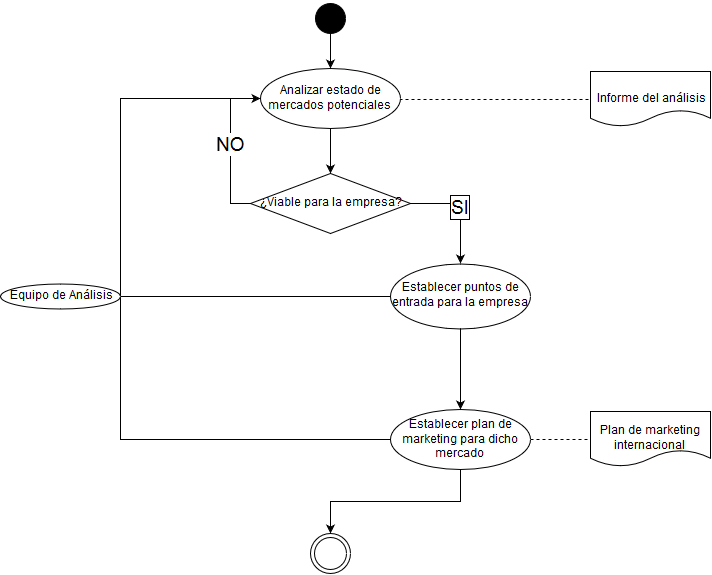
\includegraphics[width=0.75\columnwidth]{proc2} % Example image
\end{center}

\end{itemize}
\end{center}

\end{homeworkSection}
\clearpage

%----------------------------------------------------------------------------------------

\begin{homeworkSection}[f. Identificaci\'{o}n de los procseos] % Custom section title

Los procesos del apartado 1.2.d que est\'{a}n relacionados con nuestras iniciativas de gesti\'{o}n del conocimiento son los siguientes:
\begin{itemize}

\item Análisis de mercados potenciales: este proceso está relacionado con nuestra iniciativa de análisis del mercado a nivel internacional, que cubre el objetivo de potenciar el marketing internacional. Al conseguir realizar este proceso con éxito, conseguiremos aumentar la presencia internacional de nuestra empresa y por consiguiente, mejorar las ventas.

\item Análisis y reducción del impacto medioambiental del proceso de producción: este proceso está relacionado con nuestra iniciativa de crear un equipo de empleados que analice y monitorice nuestro proceso de calidad de la producción de nuestros productos. Consiguiendo realizar correctamente este proceso, conseguiremos potenciar nuestra ventaja competitiva (calidad de la producción).

\item Proceso de fabricación de los electrodomésticos: este proceso está muy relacionado tanto con el proceso anterior como con la iniciativa de análisis y mejora del proceso de fabricación. 

\item Formación de los empleados: este proceso es uno de los procesos más importantes de nuestro proceso de gestión del conocimiento, ya que para llevar a cabo las iniciativas en las que necesitamos un equipo, el conocimiento de nuestro personal tiene que estar actualizado, por lo que la formación es algo esencial.

\item Gestión adecuada de nuestros empleados: en la creación de los grupos de gestión de conocimiento para diversas iniciativas, tenemos que llevar una gestión de nuestro personal 

\item Captura de conocimiento de los empleados: Este proceso tiene gran presencia en todas las iniciativas, pero principalmente en nuestra iniciativa de crear la páginas amarillas, ya que capturar el conocimiento es un proceso importante de la iniciativa.



\end{itemize}
\end{homeworkSection}
\clearpage


%----------------------------------------------------------------------------------------
\begin{homeworkSection}[h. Identificar las fuentes externas de conocimiento] % Custom section title

\textbf{Páginas amarillas:}

Para esta iniciativa no nos hace falta ninguna fuente externa de conocimiento.

\textbf{Análisis de mercado:}
\begin{itemize}
\item Legislación: Esta fuente nos proporciona información sobre los aspectos legales del mercado y de la producción aportando los cambios y modificaciones de las leyes que rigen el comportamiento de los procesos.
\end{itemize}

\end{homeworkSection}
\end{homeworkProblem}
\clearpage


%----------------------------------------------------------------------------------------
\begin{homeworkProblem}[1.3. Estudio de viabilidad] % Custom section title

\textbf{Páginas amarillas:}
\begin{itemize}
\item Viabilidad económica: el coste económico de la creación de las páginas es mínimo comparado con su beneficio, que es muy alto ya que centraliza todo el conocimiento que tienen los empleados y lo hace más accesible.

\item Viabilidad técnica: las necesidades tecnológicas de esta iniciativa no son muy elevadas. La construcción de las páginas amarillas lleva un tiempo considerable, ya que hay que crear la herramienta para acceder a las mismas, pero los beneficios superan ampliamente a los costes. 

\item Viabilidad del proyecto: en nuestra opinión esta iniciativa es realista y se puede llevar a cabo en el tiempo adecuado para el correcto desarrollo del proceso de gestión del conocimiento.

\end{itemize}

\textbf{Análisis de mercado:}

\begin{itemize}

\item Viabilidad económica: esta iniciativa no es muy cara pero puede ser muy beneficiosa para la empresa porque si conseguimos expandirnos a otros mercados, seremos capaces de aumentar en gran medida los ingresos.

\item Viabilidad técnica: todas las necesidades tecnológicas relacionadas con esta iniciativa son mínimas ya que no hacen falta recursos extraordinarios a los que ya tiene la empresa. 

\item iabilidad del proyecto: en nuestra opinión esta iniciativa es realista y se puede llevar a cabo en el tiempo adecuado para el correcto desarrollo del proceso de gestión del conocimiento.


\end{itemize}

\end{homeworkProblem}
\clearpage

%----------------------------------------------------------------------------------------
\begin{homeworkProblem}[1.4. Definici\'{o}n de Indicadores de Gesti\'{o}n del Conocimiento] % Custom section title

\begin{itemize}
\item La Actividad: nivel de uso y aprovechamiento de los distintos procesos y canales de gesti\'{o}n del conocimiento-
Nº de usuarios, Nº de miembros, Nº de consultas...
\end{itemize}

\begin{itemize}
\item El Conocimiento: nivel de conocimiento generado y/o registrado y su nivel de consumo o aprovechamiento- 
Nº de buenas pr\'{a}cticas generadas, Nº de lecciones aprendidas generadas, Nº de ideas propuestas...
\end{itemize}

\begin{itemize}
\item Los Impactos o beneficios que se est\'{a}n obteniendo, tanto cualitativos como cuantitativos- 
Nº de personas que han mejorado su formaci\'{o}n, nº de miembros en proyectos de mejora de la calidad, Nº de casos que se resuelven con el conocimiento existente...
\end{itemize}

\textbf{Creación de páginas amarillas:}

\begin{itemize}
\item El Conocimiento: nivel de conocimiento generado y registrado y su nivel de consumo o aprovechamiento para la mejora del proceso de calidad:
\begin{itemize}
\item Nº de de buenas pr\'{a}cticas creadas y el nivel de utilizaci\'{o}n de las mismas (10/a\~{n}o)
\item Nº de lecciones aprendidas creadas a partir de las buenas pr\'{a}cticas y el nivel de utilizaci\'{o}n de las mismas (10/a\~{n}o)
\item Nº de ideas propuestas para la mejora del proceso de calidad (50/a\~{n}o)
\end{itemize}
\item La Actividad: nivel de uso y aprovechamiento de los distintos procesos y canales de gesti\'{o}n del conocimiento:
\begin{itemize}
\item Nº de usuarios que utilizan el conocimiento generado 
\item Nº de miembros que adem\'{a}s de utilizar el conocimiento, lo actualizan y mejoran 
\item Nº de consultas que se realizan a la base de datos creada 
\end{itemize}
\end{itemize}

\textbf{Análisis de mercado:}

\begin{itemize}
\item El Conocimiento: nivel de conocimiento generado y su utilizaci\'{o}n para la mejora del marketing en el extranjero
\begin{itemize}
\item Nº de de buenas pr\'{a}cticas creadas y el grado de adecuaci\'{o}n tanto para un mercado en concreto como en general
\item Nº de lecciones aprendidas creadas a partir de las buenas pr\'{a}cticas
\item Nº de ideas propuestas para la expansi\'{o}n de la empresa en el extranjero
\end{itemize}
\item La Actividad: nivel de uso y aprovechamiento de los distintos procesos y canales de gesti\'{o}n del conocimiento
\begin{itemize}
\item Nº de usuarios que utilizan el conocimiento generado
\item Nº de miembros que adem\'{a}s de utilizar el conocimiento lo aplican de manera innovadora en diferentes tipos de mercados
\item Nº de consultas que se realizan a la base de datos creada, el nivel de aprovechamiento de la misma y la expansi\'{o}n del conocimiento
\end{itemize}
\end{itemize}







\end{homeworkProblem}
\clearpage

%----------------------------------------------------------------------------------------
\begin{homeworkProblem}[2.1. Definir el ciclo de vida de GC propuesto por esta iniciativa y establecer reglas y horarios] 
El ciclo de vida del sistema de gesti\'{o}n del conocimiento propuesto comienza con la captura del conocimiento y su almacenamiento en las p\'{a}ginas amarillas. Comenzando con esta actividad conseguimos que el resto de las iniciativas sean m\'{a}s eficaces ya que los equipos encargados de llevarlas a cabo ser\'{a}n creados m\'{a}s f\'{a}cilmente y de una manera m\'{a}s \'{o}ptima. \\ \\
En segunda instancia, para las diferentes iniciativas, se crear\'{a} el equipo de gesti\'{o}n del conocimiento y este equipo se encargar\'{a} de realizar la iniciativa en concreto. \\ \\
Una vez se termine la iniciativa (la cual utilizar\'{a} el conocimiento existente en el momento actual en la empresa), se actualizar\'{a} el conocimiento introduciendo las buenas pr\'{a}cticas y las lecciones aprendidas en la realizaci\'{o}n de la misma.\\ \\
\end{homeworkProblem}

%----------------------------------------------------------------------------------------
\begin{homeworkProblem}[2.2. Definici\'{o}n de plataformas t\'{e}cnicas, el sistema de gesti\'{o}n de documentos, herramientas y t\'{e}cnicas] % Custom section title

\textbf{Analisis de mercado:}
\begin{itemize}

\item Buenas prácticas: una vez una solución es utilizada de manera consistente y sea aprobada por los expertos en el ámbito (una solución a un problema concreto que se da numerosas veces) pasará a ser considerado una buena práctica y pasará a esta sección de la plataforma implementada previamente. 
Necesitamos conocer las buenas prácticas de los mercados para poder comparar con nuestras lecciones aprendidas a la hora de decidir si los puntos de entrada son viables para nuestra empresa.

\item Lecciones aprendidas: cuando una buena práctica sea consistentemente utilizada y mejorada, pasará a formar parte de las lecciones aprendidas de la empresa. En este apartado se detallarán tanto el problema, como todas las implementaciones de soluciones que se hayan dado a lo largo del tiempo (en el estilo de un log de soluciones posibles desarrolladas a lo largo de la historia de la empresa) con la última solución (en teoría debería ser la más óptima) como la recomendada para la implementación.
Estas lecciones aprendidas son las que contrastaremos con las buenas prácticas de los diferentes mercados para determinar los mercados a tener en cuenta en el plan de marketing internacional.

\item Páginas amarillas: Aquí recogemos las fichas de conocimiento de los empleados para poder filtrar y buscar empleados por conocimiento, para así ser capaces de formar nuestro grupo de análisis de mercado con trabajadores expertos en este tipo de conocimiento.
\clearpage
\end{itemize}
\textbf{Creación de paginas amarillas}
\begin{itemize}
\item Base de datos: Guardamos información esencial para esta iniciativa en las bases de datos, desde información sobre empleados a información sobre proyectos o cursos. Usando estos datos y relaciones entre ellos podremos mostrar este conocimiento de manera oportuna en nuestra aplicación.

\item Formularios de cambios: Aquí es donde se reflejan los cambios en los datos que usa la aplicación, y después de ser confirmados se usarán para ejecutar estos cambios en las bases de datos pertinentes. De este modo, podremos mantener la base de datos correctamente actualizada sin problemas y las páginas amarillas podrán mostrar el conocimiento actualizado.

\end{itemize}
\end{homeworkProblem}
\clearpage

%----------------------------------------------------------------------------------------
\begin{homeworkProblem}[3.1. Identificaci\'{o}n del equipo GC] % Custom section title
\begin{itemize}

\item Champion: persona encargada de promover e impulsar la gesti\'{o}n del conocimiento dentro de la empresa. Es el pilar del equipo por lo que tiene que estar completamente inmerso en el proceso de gesti\'{o}n del conocimiento.
\item Representantes de las TICs: los encargados de las TIC de la empresa (tanto de las existentes como de cualquiera de las herramientas que necesitemos para el desarrollo de nuestras iniciativas)
\item Representantes de las \'{a}reas funcionales que van involucradas en las iniciativas de gesti\'{o}n del conocimiento.

\end{itemize}

No obstante existen casos específicos de equipo de GC para cada iniciativa, a continuación mostraremos los añadidos al equipo general de GC que usaremos en las 2 iniciativas:

\textbf{Análisis de mercado: }
Representantes de las áreas funcionales involucradas en los procesos de esta iniciativa, en este caso necesitaremos involucrar a empleados de RRHH para crear el grupo de análisis, que constará de representantes de los departamentos de Ventas y Marketing.

\textbf{Páginas amarillas: }
En este caso necesitaremos personal de RRHH que acceda a los datos necesarios y contribuya en la actualización de estos. También necesitaremos al departamento de IT para desarrollar y ayudar al uso/pruebas/mantenimiento de la aplicación y los datos.

\end{homeworkProblem}

%----------------------------------------------------------------------------------------
\begin{homeworkProblem}[3.2. Estrategias para la captura del conocimiento] % Custom section title

\textbf{Análisis de mercado:}
\begin{itemize}
\item Recogeremos el conocimiento tácito de nuestra propia empresa y capturaremos el conocimiento tácito de las empresas de los mercados potenciales, para así poder comparar ambos sin problemas a la hora de buscar similitudes en los mercados.

\item Análisis de las debilidades de otras empresas para poder identificar nuestras ventajas en el mercado objetivo.

ºitem Digitalización de todo el conocimiento explícito que no esté computerizado para facilitar el acceso al mismo y hacer más sencillo el proceso de la espiral del conocimiento. Para llevar a cabo esta estrategia también se utilizarán las comunidades de prácticas y lecciones aprendidas para ver si nuestras fortalezas de buenas prácticas pueden aplicarse a este nuevo mercado y a su vez detectar también los puntos débiles.

\end{itemize}

\textbf{Páginas amarillas:}

\begin{itemize}

\item Recogeremos los datos de los empleados, cursos, proyectos… usando el sistema de bases de datos, de forma que tengamos toda esta información bien estructurada y preparada para la extracción.

\item Todos los cambios de las páginas amarillas se reflejarán en los diferentes formularios de cambio que rellenarán los propios empleados, este conocimiento debe ser digitalizados para poder actualizar las bases de datos. No obstante, estos cambios deben ser confirmados por entrevistas que los empleados realizarán con los miembros del departamento de RRHH.

\end{itemize}

\end{homeworkProblem}

%----------------------------------------------------------------------------------------
\begin{homeworkProblem}[3.3. Dise\~{n}o detallado de la estructura de los documentos de cada uno de los elementos del conocimiento] % Custom section title
Los documentos que necesitaremos para el desempe\~{n}o de nuestras iniciativas son los siguientes:
\begin{itemize}
\item Buenas pr\'{a}cticas
\item Proceso + buena realizaci\'{o}n
\item Lecciones aprendidas
\item Formularios para rellenar
\item Formularios de entrevistas
\item Tests
\item Documento de alcance y viabilidad
\item P\'{a}ginas amarillas
\item P\'{a}ginas blancas
\end{itemize}
El dise\~{n}o general del encabezado de todos los documentos ser\'{a} el siguiente:
\\
\\
\begin{center}
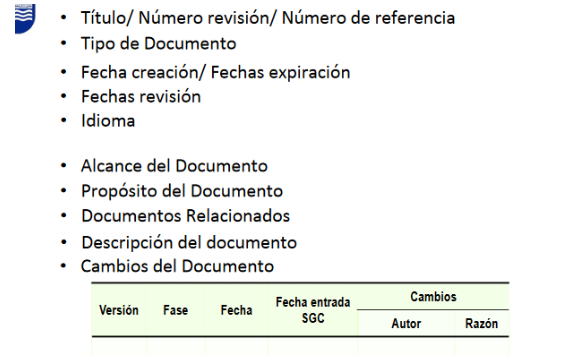
\includegraphics[width=0.75\columnwidth]{docu}
\end{center}
\clearpage

\end{homeworkProblem}
%----------------------------------------------------------------------------------------
\begin{homeworkProblem}[4.1. Formaci\'{o}n para la implementaci\'{o}n del sistema] % Custom section title
\textbf{Análisis de mercado: } para esta iniciativa, necesitaremos que nuestro departamento de marketing esté formado para poder hacer frente a cualquier oportunidad nueva de mercado y que sean capaces de aplicar el conomiento de la empresa, las buenas prácticas y las lecciones aprendidas en otras instancias para hacer frente a los nuevos desafios. 
\\
Para llevarlo a cabo, ofreceremos cursos extraordinarios fuera de los horarios de trabajo a los que nuestros empleados se podrán apuntar líbremente y que serán remunerados como horas extra. 

\textbf{Páginas amarillas: } para esta iniciativa, necesitaremos que nuestro personal de recursos humanos esté totalmente involucrado en el desarrollo diario de la empresa porque tienen que estar al día de los proyectos que se realizan para poder llevar a cabo la captura del conocimiento de una manera óptima.
\\ 
Cada dos semanas, se organizará una reunión en la cual se actualizará al personal de recursos humanos (el cual es el encargado de mantener y actualizar las páginas amarillas) de los proyectos que se están llevando a cabo en la empresa y se les pondrá al día de cuales son los objetivos de dichos proyectos. 

\end{homeworkProblem}
%----------------------------------------------------------------------------------------
\begin{homeworkProblem}[4.2. Diagrama de tiempos y actividades] % Custom section title

\textbf{Análisis de mercado: } la formación necesaria para esta iniciativa, como previamente hemos mencionado, se realizará fuera del horario laboral normal y estará remunerado como horas extra.
\\
La formación se contratará a una empresa experta en marketing y que esté especializada en el país/zona en la que está interesada la empresa o en la que se prevee que puede haber una oportunidad real de expansión. Además del conocimiento necesario sobre el estado actual del mercado tanto del país como de la región también se ofrecerá información sobre la cultura local para que nuestros empleados tengan una visión más integral de la oportunidad y del mercado objetivo.

\textbf{Páginas amarillas: } para esta iniciativa, no hace falta formación extra a la que ya poseen nuestros empleados del departamento de marketing, pero para que no pierdan los objetivos de la empresa, se realizará una reunión periódica en horario laboral en la cual se especificarán los objetivos actuales, como se están abordando y cuales son y cuales son los proyectos con los cuales se relaciona cada uno de dichos objetivos.

\end{homeworkProblem}
\clearpage
%----------------------------------------------------------------------------------------
\begin{homeworkProblem}[5. Plan para el cambio en la cultura de la Gesti\'{o}n del Conocimiento] % Custom section title

Para apoyar la implantaci\'{o}n y el uso de estas iniciativas de GC, llevaremos a cabo las siguientes acciones:
\begin{itemize}
\item Reuniones de introducci\'{o}n de iniciativas, donde se proveer\'{a} a los empleados de la informaci\'{o}n necesaria para el correcto uso e implantaci\'{o}n de estas iniciativas.
\item Como soporte a las reuniones generales para todos los empleados, tambi\'{e}\'{e}n se promover\'{a} que los encargados de cada departamento de la empresa den cursos extraordinarios por si alguna persona de su departamento necesita ayuda con el uso de las herramientas.
\item Como compensaci\'{o}n por el uso de las herramientas de gesti\'{o}n del conocimiento, se otorgar\'{a}n puntos los cuales luego se podr\'{a}n canjear por diferentes beneficios (los cuales no est\'{a}n definidos pero ser\'{a}n de tipo no econ\'{o}mico). Creemos que esta forma de compensaci\'{o}n no econ\'{o}\'{o}mica har\'{a} que se usen m\'{a}s habitualmente todas las propuestas que hemos llevado a cabo.
\end{itemize}


\end{homeworkProblem}
\clearpage
%----------------------------------------------------------------------------------------

\begin{homeworkProblem} [Anexos]
Entrevista: 
\\

Entrevista semiesteucturada
Tema: Gesti\'{o}n del proceso de producci\'{o}n de los electrodom\'{e}sticos

Hola ........., si no me equivoco pertenece al dpto.  ............., ¿Est\'{a} usted contento en su actual puesto?
\begin{itemize}
\item ¿C\'{o}mo definir\'{i}a el ambiente de trabajo en su departamento?
\item ¿Qu\'{e} otras responsabilidades le gustar\'{i}a asumir?
Entrega: Darle un texto sobre nuevas normas en la empresa, el empleado deber\'{a} extraer y explicitar los cambios necesarios a establecer en los procesos/actividades correspondientes a su puesto de trabajo.

\item ¿Le son familiares los procesos de producci\'{o}n?
\item ¿Cree usted que es necesario alg\'{u}n cambio/regulaci\'{o}n en los procesos?¿Con qu\'{e} fin?
\item ¿Tiene alg\'{u}n familiar que dependa de usted?
S\'{i} - ¿Cree usted que su trabajo presenta un obstáculo a la hora de prestar la atenci\'{o}n necesaria a esta(s) persona(s)?
\item ¿C\'{o}mo cambiar\'{i}a su situaci\'{o}n en caso de tener que cambiar a un puesto en el extranjero?¿Podr\'{i}a permitirse ese cambio?
No - ¿Tiene previsto alg\'{u}n compromiso  que pudiese propiciar esto (boda, nacimiento…)?
\item ¿Cree usted que un compromiso de este tipo podr\'{i}a conllevar cambios notorios en su rendimiento o incluso la necesidad de llevar a cabo alg\'{u}n cambio/ajuste en su puesto de trabajo?

Muchas gracias ............, ha sido un placer haber establecido esta entrevista con usted, le enviaremos el resultado de lo extra\'{i}do en el proceso para poder contrastar con su opini\'{o}n. Le llamaremos cuando finalice el proceso de entrevistas.
\end{itemize}

Entrevista estructurada
Tema: Gesti\'{o}n del proceso de producci\'{o}n de los electrodom\'{e}sticos
Hola ..........., si no me equivoco pertenece al dpto.  .............., ¿Est\'{a} usted contento en su actual puesto?
\begin{itemize}
\item ¿En su opini\'{o}n, existe un buen ambiente de trabajo dentro de su dpto.?
\item ¿Le gustar\'{i}a asumir m\'{a}s responsabilidades?
\item ¿Le son familiares los procesos de producci\'{o}n?
\item ¿Cree usted que es necesario alg\'{u}n cambio/regulaci\'{o}n en los procesos?
\item ¿Tiene alg\'{u}n familiar que dependa de usted?
S\'{i} - ¿Cree usted que su trabajo presenta un obst\'{a}culo a la hora de prestar la atención necesaria a esta(s) persona(s)?
\item ¿Presentar\'{i}a su situaci\'{o}n cambios dr\'{a}sticos en caso de tener que cambiar a un puesto en el extranjero?¿Podr\'{i}a permitirse ese cambio?
No - ¿Tiene previsto algún compromiso  que pudiese propiciar esto (boda, nacimiento…)?
\item ¿Cree usted que un compromiso de este tipo podr\'{i}a conllevar cambios notorios en su rendimiento o incluso la necesidad de llevar a cabo algún cambio/ajuste en su puesto de trabajo?

Muchas gracias ..............., ha sido un placer haber establecido esta entrevista con usted, le enviaremos el resultado de lo extra\'{u}do en el proceso para poder contrastar con su opini\'{o}n. Le llamaremos cuando finalice el proceso de entrevistas.
\end{itemize}
\end{homeworkProblem}

\end{document}
